\section{Constant Volatility}
The Black-Scholes model, introduced earlier, outlines the pricing formula for a European call option in 
Proposition \autoref{Black-Scholes Formula}. It is  essential to recall that in the Black-Scholes formula, 
volatility is considered constant. This implies that the volatility of the asset's returns does not vary over time,
establishing a direct correlation between the option's price and its volatility. Consequently, 
understanding implied volatility becomes crucial. Although the Black-Scholes model does not provide 
a closed-form solution for implied volatility, it can be determined numerically, a topic not covered 
in this analysis. Instead, we introduce the SABR model to estimate volatility, which can then be 
applied to the Black-Scholes model for option pricing.
\\\\
We will briefly demonstrate why the assumption of constant volatility does not align with market data. 
Our analysis includes examining the S$\&$P 500 index and the 10Y10Y EUR swaption, which are commonly used financial indices.
Below in \autoref{10Y10Y dev} and \autoref{sp500 dev}, respectively the develop of the 10Y10 EUR swaption and S$\&$500 index
levels is illustrated. From the two plots we see the patterns that the levels fluctuate over time. This is emphasized
if we look at \autoref{10Y10Y return} and \autoref{sp500 return}, where the return for respectively the 10Y10Y EUR 
swaption and the S$\&$P 500 index is plotted. We see that the daily return fluctuate over time, hence it doesn't look 
like the volatility in the market data is constant. So this small data analysis emphasize the point that volatility is 
not a constant figure but rather varies significantly from day to day, reflecting the market's 
response to new information and events. From the small data analysis we can deduce that the Black Scholes model 
serves as foundation tool in option pricing, but i cannot describe and capture volatility in the market. This highlights 
the necessity of models like the SABR model, which is construct to fit the market volatility better. Since The SABR model
allow for a more nuanced estimation of volatility.
\begin{figure}[h]
    \centering
    \begin{minipage}{0.5\textwidth}
        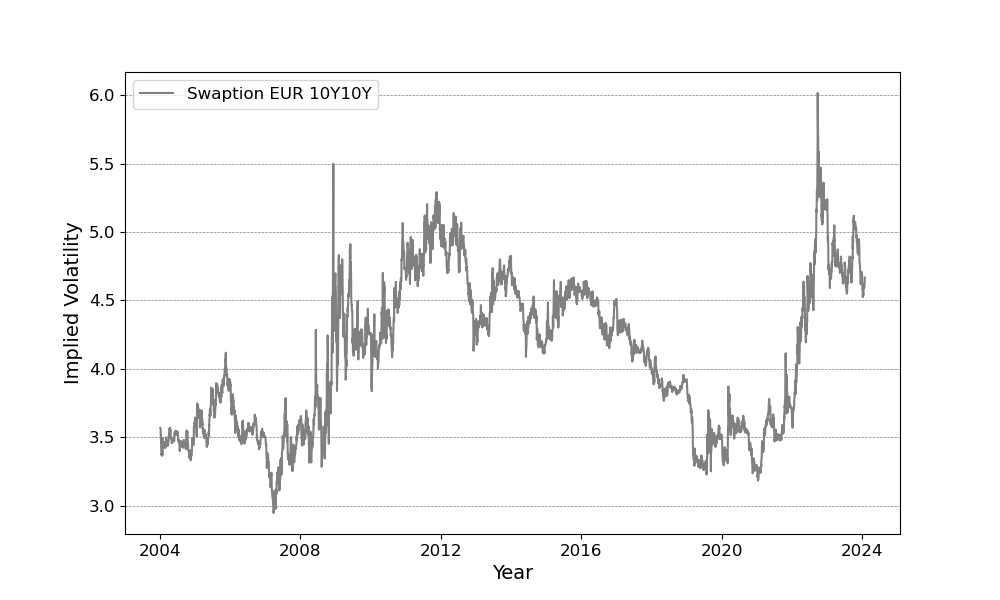
\includegraphics[width=\linewidth]{/Users/nannaingemannohrt/Desktop/master_thesis/main/plots/10Y10Yswaption.png}
        \caption{Swaption EUR 10Y10Y from  2004-01-01 \\ to 2024-01-01.}
        \label{10Y10Y dev}
    \end{minipage}\hfill 
    \begin{minipage}{0.5\textwidth}
        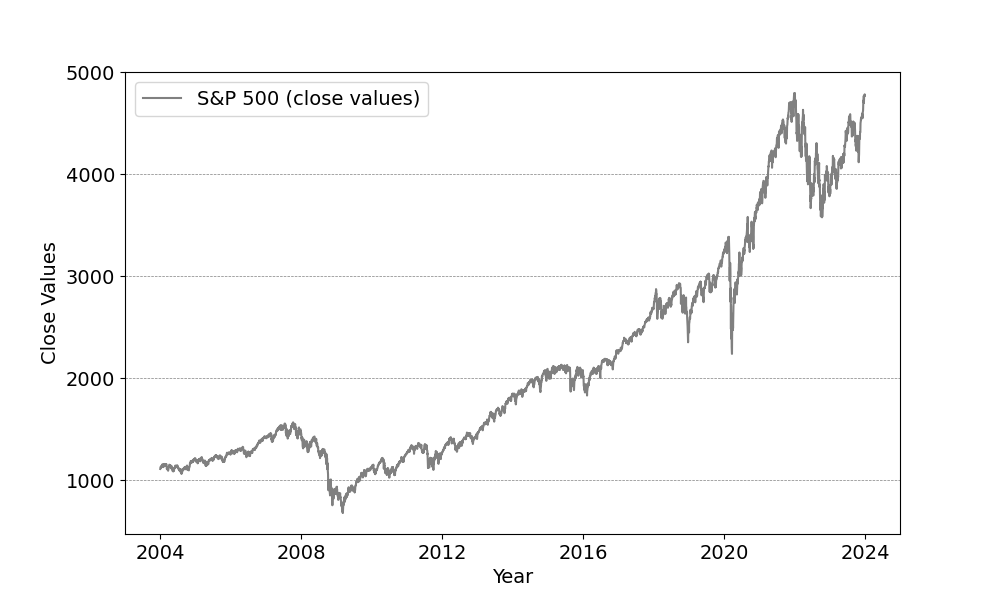
\includegraphics[width=\linewidth]{/Users/nannaingemannohrt/Desktop/master_thesis/main/plots/sp500.png}
        \caption{S$\&$P500 index (close values) from \\ 2004-01-01 to 2024-01-01.}
        \label{sp500 dev}
    \end{minipage}
\end{figure}

\begin{figure}[h]
    \centering
    \begin{minipage}{0.5\textwidth}
        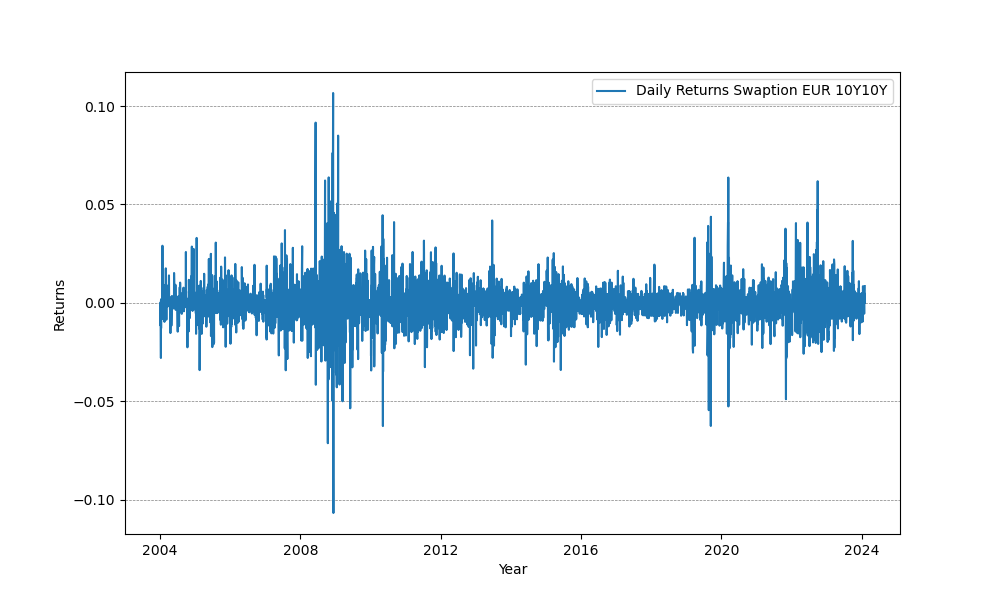
\includegraphics[width=\linewidth]{/Users/nannaingemannohrt/Desktop/master_thesis/main/plots/10Y10Yswaptionreturn.png}
        \caption{Swaption EUR 10Y10Y return from  \\ 2004-01-01 to 2024-01-01.}
        \label{10Y10Y return}
    \end{minipage}\hfill 
    \begin{minipage}{0.5\textwidth}
        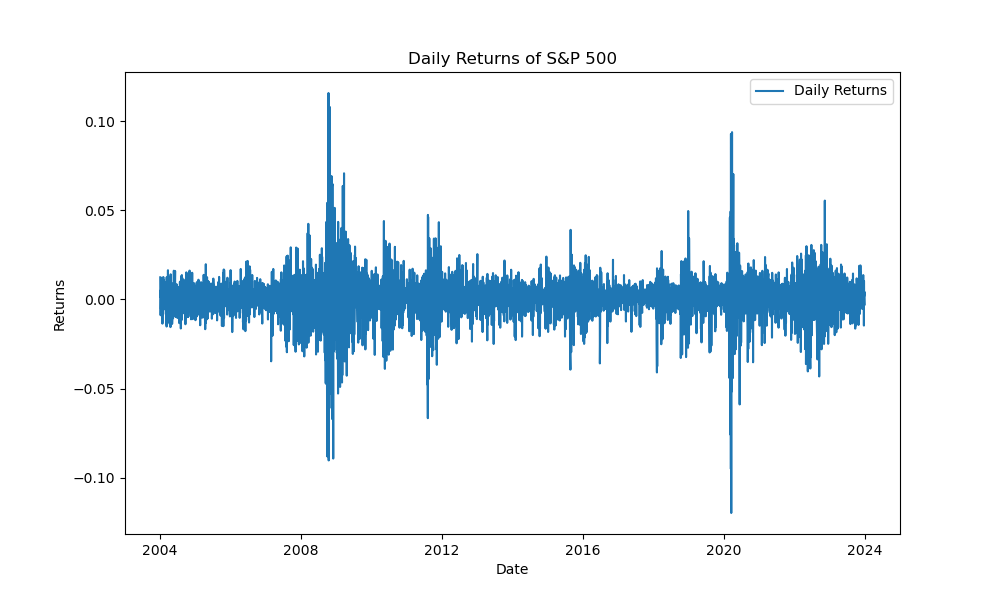
\includegraphics[width=\linewidth]{/Users/nannaingemannohrt/Desktop/master_thesis/main/plots/sp500return.png}
        \caption{S$\&$P500 index (close values) return  \\ from 2004-01-01 to 2024-01-01.}
        \label{sp500 return}
    \end{minipage}
\end{figure}